\chapter{Approach}
% Describe the performed solution with all possible details. Define necessary parameters, inputs, outputs and context of use, possible problems and when they can be applied. 

% Remember to define necessary concepts before using them, building the text from easiest definitions (not depending on previous definitions) to complex definitions (depending on previous definitions).

% E.g: 
% \begin{itemize}
%	\item Lost Communication: a lost communication occurs when the conditions of the environment are not sufficient or the distance between sender and receiver is to hight to transmit information.
%	\item Wait until rescue: when the robot loses its communication, the pre-designed state machine will stop the motors to keep the actual position. Energy safe mode will be enabled, at the same time that a channel transceiver daemon will send SOS messages every T and wait for reply during T sec. 
%\end{itemize}
% A communication efficient task scheduling system is designed to help multiple robots handle various task. 
% This system schedule task according to system resources, including system environment information, robot status and task specifications. Once this information is attained, the task scheduling system sends robot a set of task.

% \begin{itemize}
% 	\item \textbf{Robot.} Each robot is responsible for moving in 2-dimensional physical space as well as gathering measurement result from sensors. It has a rechargeable battery, and its level drops as robot moves and rotates.
% 	\item \textbf{Tasks.} Each task requires one or more robots to traverse a path in the workspace and carry out certain activitys\cite{Ivan2017}.
% 	\item \textbf{Environment.} In this project, all robots are considered moving in an office environment that contains a corridor along the central x-axis and 16 rooms located around the corridor. The environment factors, such as room locations and occupation possibilities help task scheduling.
% \end{itemize}
This chapter introduces the important concepts used in the task scheduling system. Chapter \ref{sec:architecture_design} introduces the architecture of this multi-robot system. Chapter \ref{sec:environment_and_gather_information_approach} describes the indoor office environment as well as how robot gather room occupation information. Chapter \ref{sec:task_explan} explains the definition of task as well as its composition and decomposition. Chapter \ref{sec:task_scheduling_approach} introduces the multi-robot task scheduling approach applied in the system architecture.

\section{Architecture Design}
\label{sec:architecture_design}

The architecture of the system consist of several parts: centralized pool, robot controller, navigation stack, charging station and system environment(Figure \ref{fig:system_architecture}). 

\begin{itemize}
	\item \textbf{Centralized Pool.} A centralized pool consist of several modules: multi-robot task scheduling module, map information, database, execution and monitoring. The database stores dynamic indoor environment information such as measurement result. The map information modules contain the static map information(Figure \ref{fig:database_er}). The execution and monitoring module interacts with robots. The multi-robot task scheduling module schedule tasks to robots.
	\item \textbf{Robot Controller.} A robot controller contains several modules: local task queue, execution and robot activity. The local task queue stores tasks that the robot needs to complete sequentially. The execution module receives commands from centralized pool and decides when and which task the robot should run. The robot activity module run tasks in local task queue when receives decision from execute module and interacts with environment and its navigation stack.
	\item \textbf{Navigation stack.} The move\_base node provides a ROS interface for configuring, running, and interacting with the navigation stack on a robot. It makes robot move to desired positions using the navigation stack. Its advantages include optionally performing recovery behaviors when the robot perceives itself as stuck\cite{MOVEBASE}. 
\end{itemize} 

\begin{figure}[htbp]
	\centering
	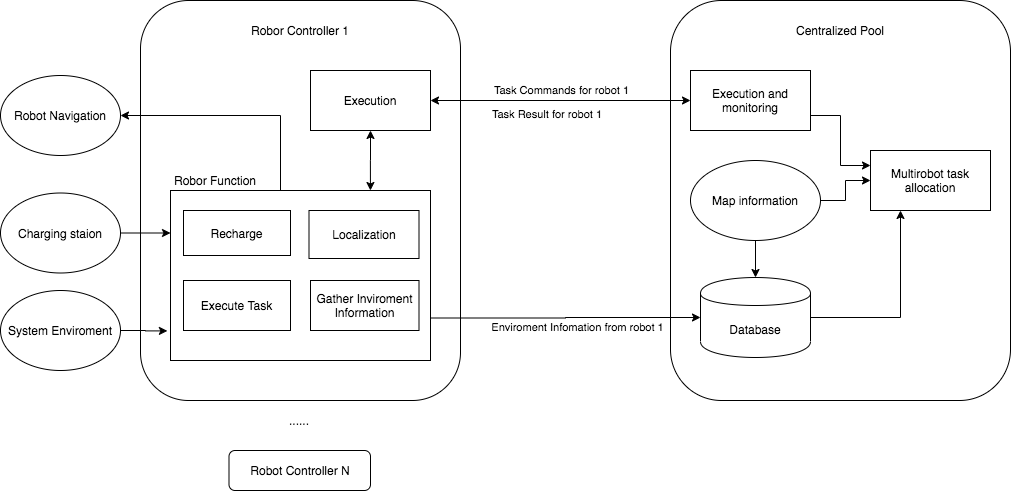
\includegraphics[width = 0.9\textwidth]{content/images/ch3/architecture.drawio.png}
	\caption{Multi-robot Task Scheduling Architecture.}
	\label{fig:system_architecture}
\end{figure}

\section{Environment and Gather Information Approach}
\label{sec:environment_and_gather_information_approach}

%\subsection{Gather Infomation Approach}
The goal of this project is to schedule tasks to robots based on the information gathered about room occupation. However, current robot sensing technology, including robots equipped with external sensors, is not good enough to gather information of whole office environment satisfactorily. 
For example, compared with office environment, the field within sensing range is rather narrow. Therefore, use of external environment information sources is essential to bridge the local knowledge gap.
In this project, since distributed IoT network cost higher than robot and its network connections consume much energy, the fixed sensors capable of short-distance communication are installed in the environment. They can share their environment information with robots, thus robots don't need to equip with numerous sensors \cite{PYO2015148}.
Robots interact with sensors while moving in the environment and report this environment information to centralized pool.
The details about centralized pool storing and studying from environment information are discussed in section \ref{sec:task_scheduling_procedure}.

%\subsection{Environment Learning}
%IoT system should be adopted in the system environment, which can provide enough environment information that help multi-robot task scheduling system to make decisions. 

%\todo{More Advantages}

\section{Tasks and Task Composition and Decomposition Approach}
\label{sec:task_explan}

\subsection{Task Specification}
Robots should navigation tasks in order to achieve the overall system goals: gather information and environmental information continuously for a long time and schedule tasks to robots based on the environmental information. Therefore, three task names are defined: ``gather information task'' asks a robot gathers environment information from sensors, ``navigation task'' asks a robot moves to a point and  ``charging task'' asks robot to refill its battery at charging station.
The task specifications are stored in ``task table'' in database (Table \ref{tab:db_task_table}).

\subsection{Task Composition and Decomposition}
Tasks can be distinguished to ``simple tasks'' and ``Complex tasks''.  ``Simple tasks'' comprises a single target position that can be performed by a single robot. A ``Complex tasks'' can be broken up or decomposed into multiple ``small tasks''. Those sub-tasks of a complex task need to be performed by the same robot.
In this project, the centralized poll not only can create ``simple tasks'' according to task specifications (Table \ref{tab:db_task_table}), but also can analyze the dependencies of ``simple tasks'' and form a dependency chain to compose ``complex tasks''. The robot (robot controller) can decompose a ``Complex task'' to ``simple tasks'' and execute ``small tasks'' according to their dependencies.

\section{Multi-robot Task Scheduling Approach}
\label{sec:task_scheduling_approach}

The multi-robot task scheduling module in the architecture should perform multi-robot task scheduling. 
The implementation of task scheduling is shown in Chapter \ref{sec:task_scheduling_procedure}. There are some general rules for multi-robot task scheduling.


\begin{enumerate}
	\item When the battery of robot below 10\%, a charging task will be created and sent to robot.
	\item When the battery of robot above 10\%, firstly, ``simple navigation tasks'' according to the task table in database are created. Secondly, ``complex navigation tasks'' will be composed and one of them will be selected and sent to robot. To ensure consistency, a ``complex task'' composed by only one ``simple task'' is allowed. 
    \item If there are no ``navigation tasks'' in database or after ``navigation tasks scheduling'', the cost of tasks exceeds the threshold, a ``gather environment task'' will be created and sent to robot.
\end{enumerate}

\subsection{Execute Task}
As discussed in Chapter \ref{sec:task_scheduling_approach}, one of the ``complex navigation tasks'' should be selected for requesting robot. In order to select an ``navigation task'', the decision variables and Equation \ref{eq:large_execute_task_cost} are used to calculate the cost. The ``complex navigation tasks'' with the lowest cost will be selected.

\begin{equation}
	\label{eq:large_execute_task_cost} 
	\begin{aligned}
	& \mbox{W: Weight } \\
	& \mbox{n: Number of doors} \\
	& \mbox{Cost}_{\mbox{Large navigation task}} = \frac{W_{\mbox{battery}} \times \mbox{Battery consumtion}}{n} + W_{\mbox{waiting}} \times \mbox{waiting time} \\
	& + W_{\mbox{probability}} \times \prod\limits_{i=1}^n \mbox{Door open probability}  + W_{\mbox{priority}} \times \mbox{Priority}
	\end{aligned}
\end{equation}

\paragraph{Decision variables}
\begin{itemize}
\item \textbf{Task Priority.}  The priority is discussed Chapter \ref{sec:task_table}.
\item \textbf{Product of Door Open Possibility.} The product of open possibilities of doors on trajectory: All doors that the robot will pass through when moving from its location to the target point.
	An example of ``measurement result'' table is shown in Table \ref{tab:db_measurement_result}, an example of ``open probability'' table is shown in Table \ref{tab:db_open_possibilities}. 
\item \textbf{Waiting Time. } The waiting time is the difference between the current simulation time and start time of the first task to be executed. $T_{waiting} = T_{first\_task} - T_{now}$
\item \textbf{Battery Consumption.} The Battery Consumption is related to robot trajectory. For a Large ``navigation task'' that contains n simple task, Equation \ref{eq:battery_consumption} can be used to calculate battery consumption. The centralized pool will send the task with the lowest cost to this robot.
\end{itemize}


\begin{equation}
\begin{aligned}
\label{eq:battery_consumption}
& \mbox{B:Battery consumption } \\
& \mbox{W: Weight } \\
& \mbox{m: Number of waypoint } \\
& \mbox{n: Number of simple task} \\
& B_{\mbox{complex task}} = \sum_{\mbox{task}_1}^{\mbox{task}_n} B_{\mbox{trajectory}} \\
& = \sum_{t = \mbox{task}_1}^{\mbox{task}_n} \sum_{\mbox{waypoint}_1}^{\mbox{waypoint}_m} [W_{\mbox{position}} \times \mbox{position variation}+W_{\mbox{angle}}  \times \mbox{angle variation}]\\
& = \sum_{t = \mbox{task}_1}^{\mbox{task}_n} \sum_{p = \mbox{waypoint}_1}^{\mbox{waypoint}_m} [ W_{\mbox{position}} \times \sqrt{(x_p-x_{p-1} )^2+(y_p-y_{p-1} )^2} \\
&   + W_{\mbox{angle}} \times 2 \times \arccos(w_p)] 
\end{aligned}
\end{equation}


\subsection{Environment Task}
As is discussed in section \ref{sec:task_scheduling_approach}, once there are no suitable tasks in centralized pool, the task scheduling module should create a ``gather environment information task'' to gather more measurement results and further more improve the accuracy of ``open possibilities'' table.
To create a ``gather environment information task'', Equation \ref{eq:door_cost} and following decision variables are used to calculate the costs of doors. A ``gather environment information task'' to the door with the lowest cost will be created.

\begin{equation}
	\label{eq:door_cost}
	\begin{aligned}
	& \mbox{W: Weight } \\
	& \mbox{n: Number of doors on trajectory} \\	
	& \mbox{Cost}_{\mbox{door}} = \frac{W_{\mbox{battery}} \times \mbox{Battery consumtion}}{n} + W_{\mbox{time}} \times (T_{\mbox{last update}} - T_{\mbox{now}}) \\
	& + W_{\mbox{probability}} \times \prod\limits_{i=1}^n \mbox{Door open probability}
	\end{aligned}
\end{equation}

\paragraph{Decision variables}
\begin{itemize}
	\item \textbf{Door Last Update Time.} The latest timestamp when the door is measured.
	\item \textbf{Product of Door Open Possibility.} The product of open possibilities of doors on trajectory: All doors that the robot will pass through when moving from its location to the front of the target door.
	\item \textbf{Battery Consumption.} The battery consumption is related to the trajectory from robot to the front of the door. Equation \ref{eq:battery_consumption} can be used to calculate battery consumption.
\end{itemize}



\subsection{Charging Task}
As is discussed in section \ref{sec:task_scheduling_approach}, once a robot sends task request to the centralized pool, the centralized pool should figure out whether this robot need charging, if yes it should create a ``charging task'' for requesting robot. 
To create a ``charging task'', Equation \ref{eq:door_cost} and following decision variables are used to calculate the costs of charging station. A ``charging task'' to the charging station with the lowest cost will be created.

\begin{equation}	
\label{eq:charging_station_cost}
\begin{aligned}
	& \mbox{W: Weight } \\
	& \mbox{Cost}_{\mbox{charging station}} = \frac{W_{\mbox{battery}} \times \mbox{battery consumtion}}{n} + W_{\mbox{time}} \times T_{\mbox{remain}}
\end{aligned}
\end{equation}


\paragraph{Decision variables}
\begin{itemize}
	\item \textbf{Remain Time.} It describes how long will a charging station be free. 
	\item \textbf{Battery Consumption.} Similar to ``navigation task'' scheduling, the battery consumption is related to the trajectory from robot to the charging station. Equation \ref{eq:battery_consumption} can be used to calculate battery consumption.
\end{itemize}

